\chapter{Preliminarii}

\section{Tipuri de învăţare automată}

Există numeroase tipuri de învăţare automată, aşa că le vom prezenta doar 
pe cele relevante lucrării noastre. De asemenea, notațiile pentru setul de 
date introduse în această secțiune vor fi folosite și în restul lucrării.

\subsection{Supervizată}

Formal, avem un set de date cu $N$ elemente, sub formă de perechi:

\begin{equation}
    S = \{(x_{1}, y_{1}), (x_{2}, y_{2}), \dots, (x_{N}, y_{N})\}
\end{equation}

unde observaţiile $x_{i} \in \mathbb{R} ^ d$ și etichetele 
$y_{i} \in \mathbb{R}$ sau $y_{i} \in \{0, 1\}$. 
Problema se reduce la 
aproximarea cât mai bună a etichetei $y_{N + 1}$ pentru o observaţie nouă 
$x_{N + 1}$.

Învăţarea \textbf{supervizată} poartă acest nume deoarece necesită supraveghere 
umană pentru a putea funcţiona. Un specialist
din domeniul actual, în cazul 
nostru, bancar, trebuie 
să parcurgă fiecare observaţie din setul de date şi să îi atribuie 
o \textbf{etichetă} corespunzătoare $y_{i}$. Acest lucru este evident dificil, având în 
vedere că seturile de date cu minim sute de mii de entităţi sunt des întâlnite.

Această metodă este folosită în probleme de clasificare sau de prezicere 
a unor fenomene.

\subsection{Nesupervizată}

Formal, avem un set de date cu $N$ elemente:

\begin{equation}
    S = \{x_{1}, x_{2}, \dots, x_{N}\}
\end{equation}

unde observaţiile $x_{i} \in \mathbb{R} ^ d$, dar nu mai apar etichetele
$y_{i}$.
În lipsa etichetelor, problema generalizată nu mai poate fi descrisă la fel 
de ușor.

Învăţarea \textbf{nesupervizată} este complementara 
celei supervizate, deci implică faptul 
că interacţiunea umană nu este necesară în pregătirea setului de date. Cu toate 
acestea, rezultatele trebuie să fie interpretate de o persoană pentru a fi relevante,
întrucât nu mai avem etichete pe care să le folosim în evaluarea automată a 
performanţei.

Această metodă este folosită pentru a grupa datele în funcţie de similaritate,
a înţelege relaţia dintre punctele din setul de date şi pentru a face o analiză 
iniţială a datelor.

Toţi algoritmii din această lucrare aparţin acestei metode de învăţare automată.

\subsection{Semi-supervizată}

Formal, avem un set de date cu $N$ elemente, partiționat în 2 mulțimi cu $N_{1}$ elemente sub formă de perechi, 
respectiv $N_{2}$ elemente:

\begin{equation}
    S_{1} = \{(x_{1}, y_{1}), (x_{2}, y_{2}), \dots, (x_{N_{1}}, y_{N_{1}})\}
\end{equation}

\begin{equation}
    S_{2} = \{x_{1}, x_{2}, \dots, x_{N_{2}}\}
\end{equation}

unde observaţiile $x_{i} \in \mathbb{R} ^ d$ și etichetele 
$y_{i} \in \mathbb{R}$ sau $y_{i} \in \{0, 1\}$. 
La fel ca în cazul supervizat, problema este în general
aproximarea cât mai bună a etichetei $y_{N + 1}$ pentru o observaţie nouă 
$x_{N + 1}$.

Învăţarea  \textbf{semi-supervizată} 
îmbină ambele paradigme prezentate anterior, astfel
că necesită un număr mic de date adnotate, lucru ce este evident mai uşor de 
obţinut faţă de un întreg set, şi un număr mare de date fara etichetă.

Această metodă este folosită spre exemplu în modelele ce se antrenează singure, 
folosind un algoritm supervizat antrenat pe datele adnotate ce este apoi 
folosit pe datele fara etichetă pentru a obţine un nou set de date adnotat.

Deşi această metodă nu este folosită în lucrarea noastră, am inclus-o deoarece 
ideea de bază în novelty detection cu metode nesupervizate este similară. Nu avem 
nevoie de date adnotate la antrenare şi este suficient un set mic pentru testarea 
ulterioară a performanţei.


Mai jos prezentăm algoritmii pentru detectarea anomaliilor folosiţi în această lucrare.


\section{One Class SVM cu kernel}

\subsection{Ideea algoritmului}

Această metodă este inspirată din clasificatorul cu vectori suport. Ideea este 
sa găsim \textbf{un hiperplan cu margine maximă}, posibil într-un spaţiu cu 
mai multe dimensiuni decât cel iniţial, în funcţie de kernel,
care să separe originea (se presupune că punctele sunt centrate) spaţiului de trăsături
de restul punctelor din setul de date\cite{scholkopf2000support}.

Un alt mod de a privi algoritmul este găsirea celei mai \textbf{mici 
hipersfere} care să includă toate punctele din setul de date\cite{tax2004support}.

\begin{figure}[H]
    \centering
    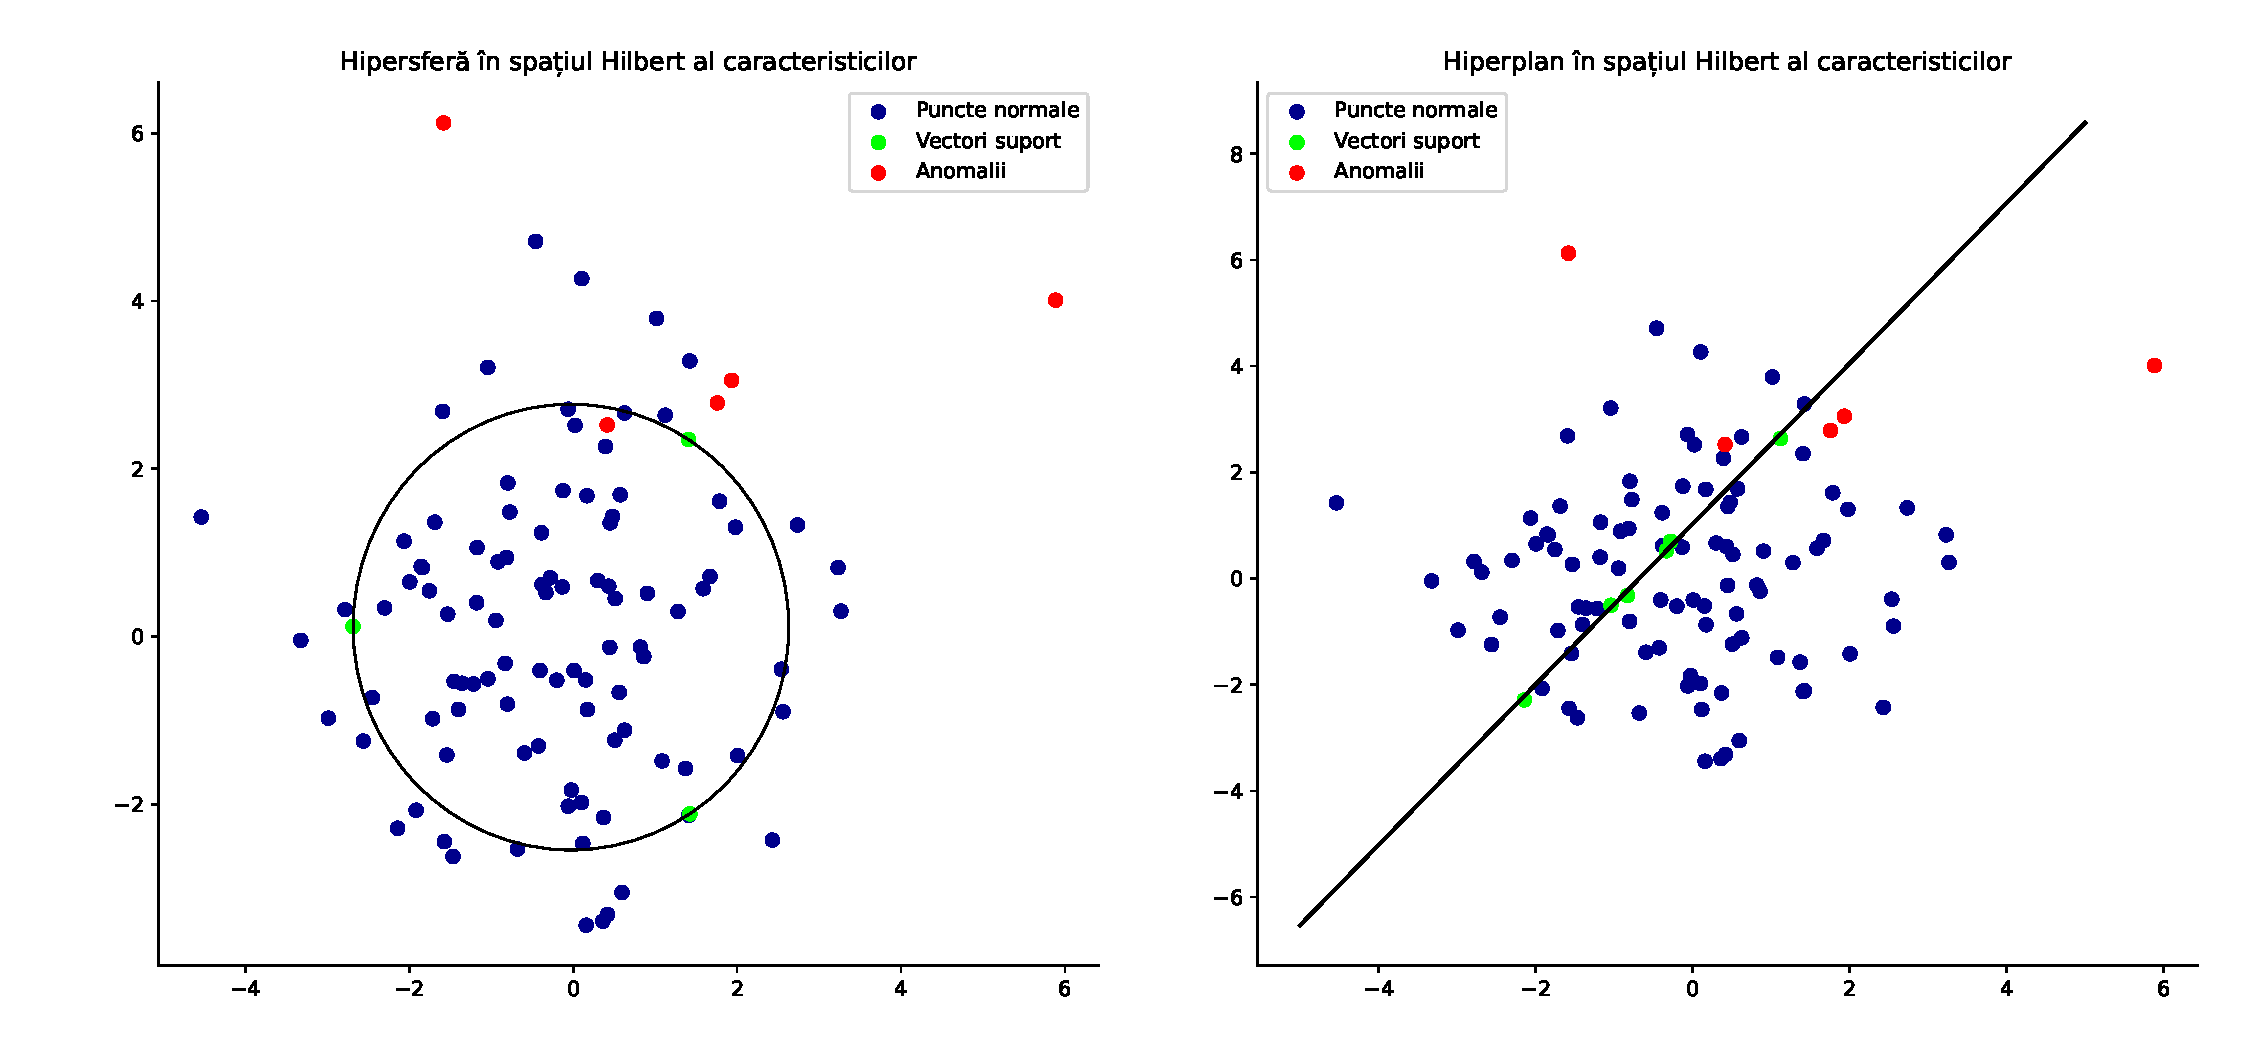
\includegraphics[width=\linewidth]{images/cvx_ocsvm_figures.pdf}
    \caption{Varianta Schölkopf et al în dreapta şi varianta Tax et al în stânga.
        Punctele roşii reprezintă anomaliile adevărate. 
        $N=105$ puncte şi $d=2$ atribute.
    }
\end{figure}

\section{Caracteristici}

One Class SVM ne ajută să transformăm un model de clasificare 
cu mai multe clase, anume SVM, într-unul cu o singură clasă,
păstrând posibilitatea de a putea introduce neliniarități 
cu ajutorul funcţiilor de kernel ce au fost studiate extensiv.
Prin urmare, One Class SVM are majoritatea avantajelor celui din urmă, precum
garanția optimului global datorită funcţiei convexe pe care
o minimizăm. Pentru problemele neconvexe, probabilitatea de 
a găsi o soluție la o distanță acceptabilă de optimul global, în general, 
scade cu creşterea dimensionalității. Mulţumită convexităţii, 
nu apare această dificultate la One Class SVM. De asemenea, 
algoritmul poate fi folosit eficient chiar și dacă 
numărul de caracteristici al punctelor din set este mai
mare decât cardinalul setului, datorită complexității de timp 
polinomiale.

Totuşi, acest model devine imposibil de folosit pentru 
seturi mari de date, complexitatea de timp lasă de dorit 
la antrenare, iar găsirea hiperparametrilor optimi este 
dificilă, atât din lipsa unor euristici bune după care 
să ne ghidăm în căutarea acestora, dar și din faptul că verificarea 
unui număr mare de combinații de hiperparametri  
ar dura prea mult din cauza complexității de timp ridicate 
la antrenare. De asemenea, rezultatele date de acest model 
nu pot fi ușor interpretate. Acestea reprezintă distanţele punctelor 
faţă de graniţa de separare, iar scorurile de anomalie sunt decise 
în funcţie de distanţele menţionate anterior, dar ele nu sunt probabilități.

\subsection{Formularea matematică}

Prima formulare ce implică un hiperplan de separare

\begin{equation}
    \begin{aligned}
    & \underset{w, \rho, \xi}{\text{min}}
    & & \frac{1}{2} \|w\|^2 + \frac{1}{\nu N} \sum_{i=1}^{N} \xi_i - \rho \\
    & \text{cu constrângerea}
    & & \langle w, \phi(x_i) \rangle \geq \rho - \xi_i, \quad i=1,2,\ldots,N \\
    &&& \xi_i \geq 0, \quad i=1,2,\ldots,N \\
    \end{aligned}
    \end{equation}
    
    \begin{itemize}
        \item $w$ este vectorul de pondere al hiperplanului
        \item $\rho$ este termenul de influenţă
        \item $\xi_i$ sunt variabilele de relaxare pentru încălcarea marginii
        \item $\phi(x_i)$ este funcţia de scufundare pentru $x_i$.
        \item $N$ este numărul total de puncte
        \item $\nu$ este marginea superioară pentru ponderea de anomalii şi marginea 
        inferioară pentru ponderea de vectori suport
    
    \end{itemize}


    Forma sa duală implică folosirea unei funcţii kernel pentru găsirea unui hiperplan 
    de separare într-un spaţiu cu mai multe dimensiuni decât cel iniţial


    \begin{equation}
        \begin{aligned}
        & \underset{\alpha}{\text{min}}
        & & \frac{1}{2} \sum_{i=1}^{N} \sum_{j=1}^{N} \alpha_i \alpha_j K(x_i, x_j) \\
        & \text{cu constrângerea}
        & & 0 \leq \alpha_i \leq \frac{1}{\nu N}, \quad i=1,2,\ldots,N \\
        &&& \sum_{i=1}^{N} \alpha_i = 1
        \end{aligned}
        \end{equation}
    
    \begin{itemize}
        \item $\alpha_i$ sunt variabilele duale asociate punctelor 
        \item $K(x_i, x_j)$ este funcţia kernel
    \end{itemize}

A doua formulare ce implică găsirea hipersferei minime

    \begin{equation}
        \begin{aligned}
        & \underset{R, c, \xi}{\text{min}}
        & & R^2 + \frac{1}{\nu N} \sum_{i=1}^{N} \xi_i \\
        & \text{cu constrângerea}
        & & \|\phi(x_i) - c\|^2 \leq R^2 + \xi_i, \quad i=1,2,\ldots,N \\
        &&& \xi_i \geq 0, \quad i=1,2,\ldots,N \\
        \end{aligned}
        \end{equation}
        
        \begin{itemize}
        \item $R$ este raza hipersferei
        \item $c$ este centrul hipersferei
        \end{itemize}
      
        
\subsection{Tehnici de optimizare}

Toate funcțiile prezentate mai sus sunt convexe, iar constrângerile 
lor sunt mulțimi convexe. Chiar
și prima constrângere din formularea cu hipersferă
care conține un termen la pătrat în dreapta 
inegalității poate fi redusă la o constrângere liniară
introducând o nouă variabilă $R_2 = R ^ 2$ cu constrângerea 
$R_2 \geq 0$.

Deci știm că problemele de optimizare
sunt convexe și astfel avem garanția unui unic minim global. 
Prin urmare, putem folosi 
tehnicile populare de optimizare convexă.

O metodă des întâlnită de ordinul întâi este coborârea pe gradient ce este 
avantajoasă atunci când setul de  antrenare este mare, întrucât 
complexitatea algoritmului nu depinde de mărimea setului de date.
Totuşi, această tehnică întâmpină dificultăţi la optimizarea funcţiilor 
cu constrângeri. Există modificări ale tehnicii de bază, precum coborârea pe 
gradient proiectată care poate lucra şi cu constrângeri liniare simple sau 
algoritmul Pegasos\cite{Pegasos} care poate rezolva varianta primitivă a primei forme prezentate 
mai sus, dar pentru formulările complexe nu se poate aplica această metodă.

În majoritatea cazurilor, un alt kernel decât cel liniar va fi folosit, şi prin urmare 
vor apărea următoarele dificultăţi: calcularea valorilor funcţiei kernel este 
o operaţie costisitoare, calcularea matricei kernel este de cele mai multe ori 
inutilă, întrucât ne interesează doar calculele ce implică un vector suport, şi 
matricea kernel de cele mai multe ori nu va încăpea în memorie din cauza 
numărului excesiv de exemple de antrenare, având în vedere că dimensiunea ei 
este de $N\times N$\cite{SVM-solvers}.

Astfel, apare nevoia unor algoritmi specializaţi. Cel mai popular dintre ei 
este SMO\cite{SMO} care foloseşte tehnici de programare pătratică şi care utilizează 
o descompunere în 
subprobleme mai mici ce pot fi rezolvate eficient şi care încap în memorie.
O implementare a acestei metode se poate găsi în biblioteca LIBSVM\cite{LIBSVM}.


\section{Gaussian Mixture Model}

\subsection{Ideea algoritmului}

Este prea restrictiv să presupunem că fiecare punct dintr-un set de date 
provine din aceeaşi distribuţie unimodală. Prin urmare, a apărut tehnica de bază 
\textbf{"Mixture model"} ce îşi propune să elimine presupunerea anterioară pentru 
a putea modela şi distribuţii multimodale care poate nu provin nici măcar din aceeaşi 
familie, utilizând o sumă ponderată de mai multe componente cu proprietăţi
cunoscute. Totuşi, în practică, se folosesc componente din aceeaşi familie pentru 
modelarea distribuţiei doar că fiecare componentă are parametri diferiţi.

Algoritmul încearcă să estimeze funcţia densitate de probabilitate 
din care au fost generate datele folosind 
\textbf{mai multe distribuţii Gaussiene}.
Astfel, putem modela distribuţii multimodale utilizând o distribuţie bine cunoscută.
Parametrii necesari sunt mediile, matricele de 
covarianţă și ponderile fiecărei componente.

Metoda este similară cu \textbf{k-means}, întrucât ambele folosesc 
măsuri de similaritate pentru a crea grupuri
ce modelează datele. Totuşi, față de k-means,
Gaussian Mixture Model permite unui punct să aparțină 
mai multor grupuri, oferind probabilități pentru fiecare,
și poate modela chiar și seturi de date complexe 
cu margini de decizie neliniare.

\begin{figure}[H]
    \centering
    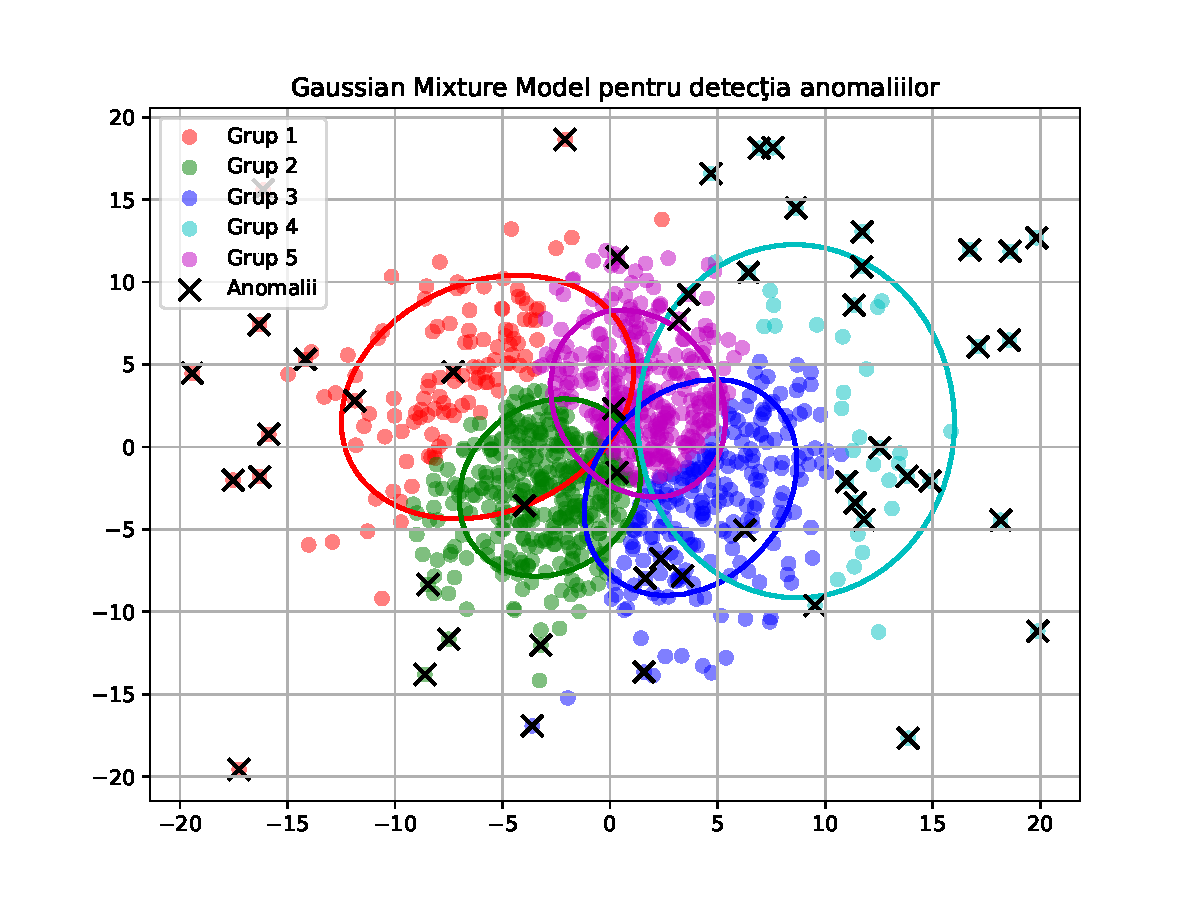
\includegraphics[width=\linewidth]{images/gmm_anomalies.pdf}
    \caption{Detecţia anomaliilor cu $K=5$ componente Gaussiene.
    $N=1050$ puncte cu $d=2$ atribute.}
\end{figure}

\section{Caracteristici}

Gaussian Mixture Model este util pentru modelarea distribuţiilor 
complexe și se descurcă bine chiar și când setul de date 
este compus din mulțimi suprapuse de puncte, întrucât află 
pentru fiecare componentă probabilitatea ca o observaţie
să fie membra acesteia, deci chiar dacă un punct se află 
în mai multe mulțimi, nu va fi repartizat doar în una singură.
De asemenea, timpul de antrenare este redus chiar și pentru 
seturi mari de date datorită tehnicii iterative de optimizare 
utilizată.

Din păcate, numărul de componente nu este ușor de ales 
pentru a obține un model optim, iar performanţa algoritmului 
depinde foarte mult de inițializarea parametrilor iniţiali, 
ceea ce poate duce la imposibilitatea convergenței către optim.
De asemenea, se presupune că datele pot fi modelate de o 
combinație de distribuţii Gaussiane, dar dacă acest lucru 
nu este adevărat, algoritmul nu va oferi rezultate bune.

Pentru reducerea numărului de parametri ce trebuie învățați,
se poate face presupunerea că caracteristicile datelor 
sunt independente unele de altele. Acest lucru este 
echivalent cu presupunerea că valorile ce nu se află 
pe diagonala principală a matricelor de covarianţă
pot fi considerate 0, dar în practică, datele pot 
fi corelate de-a lungul diferitelor dimensiuni, ceea 
ce ar conduce la învăţarea unui număr de $d^2$ parametri 
pentru fiecare componentă, unde $d$ este dimensiunea unui punct.
Acest lucru ar putea duce la overfitting când setul de date 
este mic\cite{aggarwal2017outlier}.
Un alt dezavantaj este vulnerabilitatea la blestemul 
dimensionalității.

\subsection{Formularea matematică}

Funcţia densitate de probabilitate estimată este dată de

\begin{equation}
    \text{p}(x) = \sum_{i=1}^{K} \phi_i \mathcal{N}(x|\mu_i, \Sigma_i)
\end{equation}

\begin{itemize}
    \item $K$ este numărul de componente Gaussiene
    \item $\mathcal{N}(x | \mu_i, \Sigma_i)$ este distribuţia Gaussiană
    cu medie $\mu_i$ şi matrice de covarianţă $\Sigma_i$
    \item $\phi_i$ este ponderea componentei $i$
\end{itemize}

Totuşi, pentru a detecta anomalii avem nevoie de 

\begin{equation}
    p'(x) = 1 - \prod_{i=1}^{K} \left(1 - p_k(x)\right)
\end{equation}
    
\begin{itemize}
    \item $p_k(x)$ este probabilitatea ca punctul $x$ să 
    aparțină componentei $k$
\end{itemize}

Această formulă ne indică probabilitatea ca un punct să fi fost generat de oricare 
dintre componentele Gaussiene implicate. Deci, o valoare cât mai mică sugerează 
o şansă mare ca punctul să fie anomalie.

\subsection{Tehnici de optimizare}

Pentru Gaussian Mixture Model nu se poate găsi nicio 
soluție în formă închisă din cauza faptului că 
valorile optime ale parametrilor depind de probabilitatea 
datelor de a aparține fiecărei componente, dar în același 
timp, calcularea acestor probabilități depinde de 
parametrii optimi.

Prin umare, este nevoie de o soluție iterativă care 
aproximează alternativ valorile căutate mai sus.
Cea mai populară metodă este algoritmul 
\textbf{Expectation-Maximization} (EM). Acesta este compus din 
2 pași care sunt repetați până când eroarea față de 
soluția optimă scade sub un anumit prag. La pasul $E$,
folosim valorile actuale ale parametrilor pentru a 
calcula probabilitatea că un punct a fost generat 
de o anumită componentă, făcând acest lucru pentru 
toate punctele și toate componentele. La pasul $M$,
utilizăm probabilităţile calculate la pasul $E$ 
pentru a estima valorile parametrilor optimi 
cu metoda \textbf{Maximum Likelihood Estimation} care caută 
să maximizeze probabilitatea de observare a datelor 
sub un anumit model statistic.

Numărul de componente poate fi ales ori folosind anumite 
criterii, precum \textbf{Bayesian information criterion} 
și \textbf{Akaike information criterion}, 
ori folosind cunoștințe 
din domeniul problemei.

Pentru inițializarea parametrilor se poate folosi 
algoritmul k-means. Acesta ne va da direct valori 
inițiale pentru mediile grupurilor. Pentru matricele 
de covarianţă putem folosi covarianţele calculate 
pentru punctele din fiecare grup, iar pentru ponderi 
vom folosi proporția de puncte din setul de date
aparținând fiecărui grup\cite{EM-GMM-INIT}.

\section{Kernel Density Estimation}

\subsection{Ideea algoritmului}

Precum Gaussian Mixture Model, algoritmul încearcă să estimeze 
funcţia densitate de probabilitate din care au fost generate datele.

Tehnica de bază utilizează un kernel funcţie de distribuţie probabilitate
pe care "îl plasăm" la fiecare punct din setul de date, căruia îi oferim o pondere 
de $\frac{1}{N}$, unde $N$ este numărul de observaţii. Apoi, distribuţia adevărată
este aproximată prin adunarea tuturor rezultatelor precedente. Procesul este similar 
aflării ariei de sub graficul unei funcţii cu ajutorul unei integrale ce 
apare dintr-o sumă de valori ale funcţiei într-o infinitate de puncte.

Altă tehnică similară de estimare a funcţiei densitate de 
probabilitate este cea a \textbf{histogramelor}
care se bazează
pe discretizarea datelor în coșuri de mărime fixă. 
Totuși, acest lucru irosește informația despre 
locațiile individuale ale punctelor, înlocuindu-le 
cu intervale ce corespund mai multor puncte. 
Astfel, graficul funcţiei va deveni discontinuu și 
constant pe fiecare interval. Kernel Density Estimation 
produce un grafic neted de cele mai multe ori și 
oferă o reprezentare mai bună a distribuției unei variabile 
continue\cite{KDE_paper}.

Un parametru numit \textbf{"lăţime de bandă"} influenţează netezimea distribuţiei 
rezultate.
Cel mai des utilizat kernel este cel Gaussian şi pe acesta îl vom folosi şi noi.

Aici, pentru fiecare punct generăm o distribuţie Gaussiană cu \textbf{media} egală
cu punctul respectiv şi \textbf{deviaţie} egală cu "lăţimea de bandă". Apoi, adunăm toate 
distribuţiile obţinute mai sus si le împărţim la numărul total de puncte.

\begin{figure}[H]
    \centering
    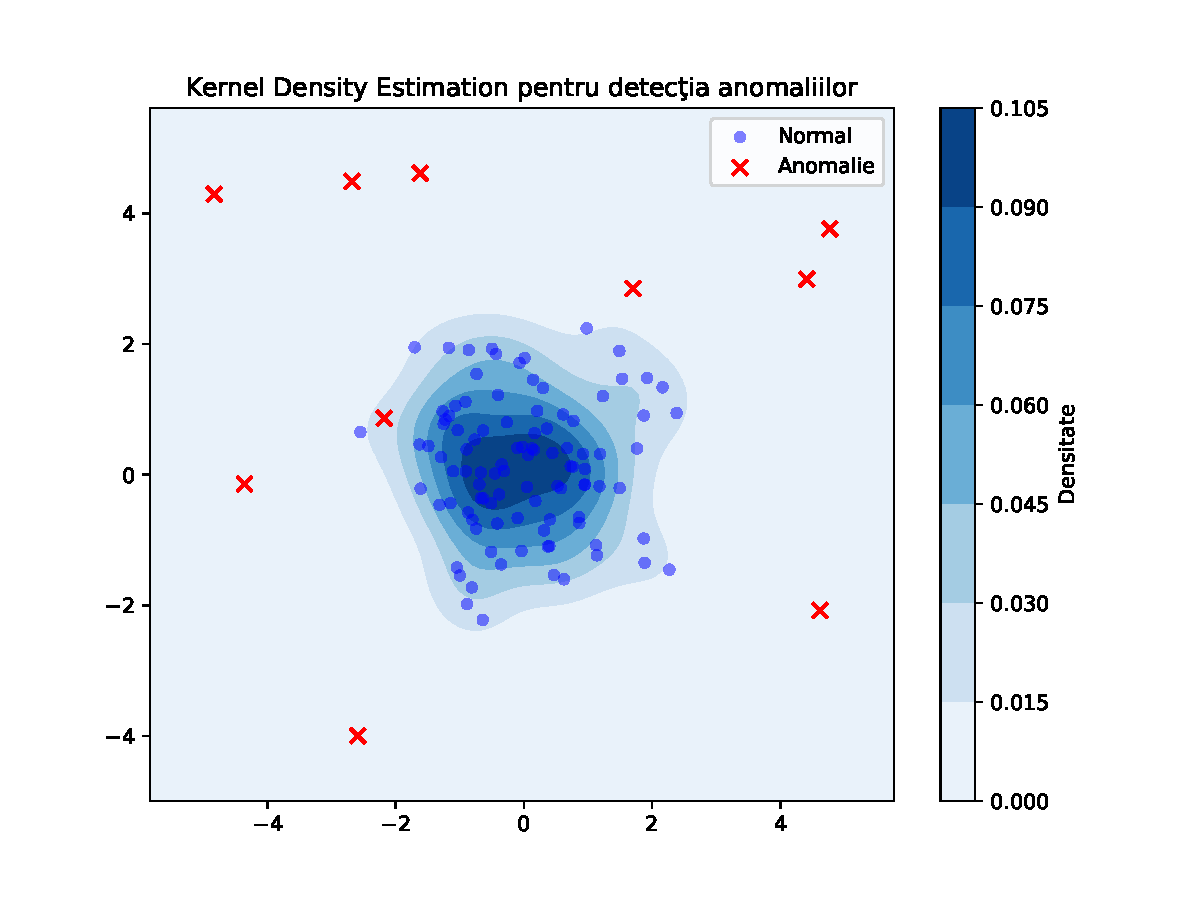
\includegraphics[width=\linewidth]{images/kde_anomalies.pdf}
    \caption{Anomaliile sunt reprezentate de punctele roşii.
    $N=110$ puncte cu $d=2$ atribute.}
\end{figure}

\section{Caracteristici}

Kernel Density Estimation are avantajul de a fi o metoda 
neparametrică și care nu face nicio presupunere asupra 
distribuţiei reale a datelor, ceea ce îl face flexibil 
pentru diverse tipuri de date. De asemenea, rezultatele 
sunt ușor de interpretat acestea fiind probabilități și 
beneficiem de informație locală despre
densitatea datelor în jurul fiecărui punct 
din set, ceea ce ne ajută la găsirea regiunilor cu densitate ridicată 
sau scăzută.

Dezavantajele sunt găsirea dificilă a hiperparametrului 
optim pentru 
lăţime de bandă, complexitatea de timp crescută, în special 
pentru seturi de date mari, vulnerabilitatea la blestemul 
dimensionalității, dar și tendința de a atribui o densitate 
ridicată punctelor din marginea setului de date, chiar 
dacă distribuţia nu se mai întinde în direcția respectivă, 
iar acest lucru poate duce la netezirea excesivă a marginilor 
distribuţiei.

\subsection{Formularea matematică}

Densitatea estimată de kernel într-un punct $x$ este dată de

\begin{equation}
\hat{f}_h(x) = \frac{1}{nh} \sum_{i=1}^{N} K\left(\frac{x - x_i}{h}\right)
\end{equation}

\begin{itemize}
    \item $N$ este numărul total de puncte
    \item $h$ este lăţimea de bandă
    \item $K(u)$ este funcţia kernel 
\end{itemize}

\subsection{Tehnici de optimizare}

Kernel Density Estimation este un model din familia celor care 
se bazează pe utilizarea unui număr finit 
dintre cei mai apropiaţi vecini ai unui punct pentru a lua 
o decizie. Pentru a cuantifica cât de apropiate sunt 2 puncte, 
se pot folosi oricare dintre metricile populare, precum distanța 
euclidiană, sau funcţiile kernel în cazul acestui model, spre exemplu.

Apartenenţa la această familie de algoritmi implică nevoia de a memora
setul de date pe care este antrenat, etapa de învăţare, practic, nefiind 
existentă. Totuşi, o abordare cu forţă brută ar necesita calcularea 
funcţiei kernel între toate perechile de puncte memorate şi cele pentru 
care dorim să aflăm densitatea de probabilitate, adică o complexitate de timp 
de $O(NM)$, unde $N$ este numărul total de puncte şi $M$ este numărul de puncte 
evaluate.

O îmbunătăţire ar putea fi utilizarea unei structuri de date ce oferă 
căutari rapide ale punctelor într-un anumit spaţiu, precum \textbf{KD Trees} 
şi \textbf{Ball trees}, aceasta din urmă fiind adesea utilizată pentru date cu 
dimensiuni $d < 20$. Pentru seturi de date mici sau pentru cazurile în care 
ne dorim să evaluăm un număr $M$ mic de puncte, este mai util să folosim forţa 
brută, întrucât crearea arborilor din KD Trees şi Ball trees 
poate dura mai mult decât simpla calculare a funcţiei kernel între toate 
perechile. În restul cazurilor însă, timpul de preprocesare devine amortizat 
de evaluările ce se pot face în timp $O(M\log(N))$. Implementări pentru 
aceste structuri de date se găsesc în biblioteca scikit-learn\cite{scikit-learn}.

Pentru acest model nu este prea relevantă funcţia kernel aleasă, 
hiperparametrul $h$ fiind cel care influenţează mai mult performanţa.

Metodele 
prezentate mai sus pot estima funcţia de densitate probabilitate doar 
pentru un singur $h$. Dacă dorim să testăm performanţa pe mai multe valori $h$, 
trebuie să rulăm acei algoritmi de mai multe ori. Acest lucru va duce la o perioadă 
mult prea mare de căutare a hiperparametrului 
în lipsa resurselor de calcul necesare 
pentru a paraleliza procesul.

Astfel, a apărut şi o variantă generalizată a modelelor ce foloseau un 
$h$ fix, menită să scadă timpul de căutare a valorii optime pentru lăţimea 
de bandă\cite{Rapid-KDE}.

\section{Metrici de performanţă}

Setul de date prezentat în această lucrare este adnotat în întregime, aşa 
că putem folosi aceleaşi tehnici de evaluare a performanţei utilizate pentru
clasificarea binară.

Prin urmare, are sens să folosim următoarele noţiuni ce vor fi utile pentru
descrierea metricilor de performanţă prezentate mai jos:

\begin{itemize}
    \item \textbf{TP} (\textit{true positive}) - reprezintă observaţiile din clasa 
    \textbf{pozitivă} ce au fost clasificate \textbf{corect}
    \item \textbf{TN} (\textit{true negative}) - reprezintă observaţiile din clasa 
    \textbf{negativă} ce au fost clasificate \textbf{corect}
    \item \textbf{FP} (\textit{false positive}) - reprezintă observaţiile din clasa 
    \textbf{pozitivă} ce au fost clasificate \textbf{greşit}
    \item \textbf{FN} (\textit{false negative}) - reprezintă observaţiile din clasa 
    \textbf{negativă} ce au fost clasificate \textbf{greşit}
\end{itemize}
În cazul nostru, clasa \textbf{pozitivă} este reprezentată de \textbf{anomalii}, iar 
clasa \textbf{negativă} este reprezentată de datele \textbf{normale}.

Metricile descrise în această lucrare reprezintă o alegere personală pe care o facem, astfel
încât să reflecte cât mai bine nevoile problemei expuse şi nicidecum nu reprezintă singura
sau cea mai bună cale de a evalua performanţa algoritmilor. Putem pune în paralelă cu teorema
\textbf{"No Free Lunch"} care ne spune că nu există un model care să fie cel mai bun în toate situaţiile,
ci că utilitatea acestuia depinde strict de context. La fel este şi în cazul măsurilor de evaluare,
iar acest fapt face găsirea uneltei potrivite pentru problemă una nu tocmai simplă, ba chiar 
poate necesita un timp considerabil de gândire.

\subsection{Accuracy}

\begin{equation}
    \text{Accuracy} = \frac{TP + TN}{TP + TN + FP + FN}
\end{equation}

Această metrică ne indică câte 
\textbf{clasificări făcute de model au fost corecte din 
totalul de puncte care trebuie clasificate}.

\subsection{Precision}

\begin{equation}
    \text{Precision} = \frac{TP}{TP + FP}
\end{equation}

Precision ne indică \textbf{capacitatea modelului de a nu produce fals pozitive}, în cazul nostru,
de a nu raporta o valoare normală ca fiind anomalie.

\subsection{Recall}

\begin{equation}
    \text{Recall} = \frac{TP}{TP + FN}
\end{equation}

Recall ne indică 
\textbf{capacitatea modelului de a identifica toate observaţiile pozitive},
în cazul nostru, de a detecta toate anomaliile.

\subsection{F1 score}

\begin{equation}
    \text{F1 Score} = \frac{2 \cdot \text{Precision} \cdot \text{Recall}}{\text{Precision} + \text{Recall}}
\end{equation}

F1 score reprezintă \textbf{media armonică dintre precision şi recall}. Prin urmare, f1 score 
va tinde către valoarea mai mică dintre aceste 2 metrici. Pentru a o maximiza,
ar trebui sa avem o valoare mare atât pentru precision, cât şi pentru recall,
fapt ce ar duce la un model ideal.

\subsection{AUC şi Curba ROC}

Curba ROC ne ajută să evaluăm calitatea modelului prin reprezentarea grafică 
a ratei de fals pozitiv pe axa X şi a ratei de adevărat pozitiv pe axa Y. 
\textbf{Punctul 
ideal al graficului se află în colţul din stânga sus} pentru ca ne dorim o 
rată de fals pozitiv egală cu 0 şi o rată de adevărat pozitiv egală cu 1. Prin urmare,
ne dorim să maximizăm rata de adevărat pozitiv şi de a minimiza rata de fals pozitiv.

Pentru a crea graficul, avem nevoie de \textbf{probabilităţile sau valorile de încredere} 
pentru fiecare observaţie din setul de  testare, generate de funcţia de decizie a 
modelului respectiv. Punctele de pe grafic pot fi văzute precum clasificatoare 
separate ce diferă prin \textbf{pragul} aplicat funcţiei de decizie. Prin urmare, dacă
dorim să ilustrăm Curba ROC, avem nevoie de un algoritm ce are ca valori de ieşire
scoruri care pot fi comparate. One Class SVM, prin definiţie, nu oferă astfel de 
rezultate, aşa că va trebui să îl tratăm în mod diferit.

\textbf{Funcţia de decizie} este cea care atribuie un scor pentru 
un punct din set cu scopul de a indica nivelul de normalitate sau de anomalie 
al acestuia. Generarea etichetei se face apoi folosind un prag în cazul 
probabilităţilor, precum Gaussian Mixture Model şi Kernel Density Estimation, 
sau efectiv reducând valorile pozitive la $+1$ şi pe cele negative la $-1$,
precum One Class SVM.

Totuşi, Curba ROC are caracter vizual şi nu ne oferă o măsură concretă a performanţei.
De aceea, avem nevoie de \textbf{AUC}, valoare ce reprezintă aria de sub grafic. Cu cât aria
este mai mare, cu atât modelul este mai bun.

\subsection{Micro average vs Macro average}

Aceste 2 tehnici pot fi folosite și în cazul clasificării cu 2 clase, dar 
ele au apărut în principal pentru a servi ca generalizare a metricilor 
clasice de performanţă care de unele singure tratează 
doar cazul \textbf{One-versus-All}, anume 
când considerăm că există doar 2 clase,
una care conține clasa țintă și una care 
conține toate celelalte clase diferite de cea din urmă. Astfel, putem 
combina măsurile de evaluare deja existente pentru a obține 
rezultate relevante în cazul general.

Nu există o singură metodă de evaluare a modelelor care să fie potrivită în toate 
cazurile. În schimb, metodele sunt alese astfel încât să reflecte cât mai bine 
nevoile problemei.

\textbf{Macro} average pentru o măsură de evaluare are forma:

\begin{equation}
    B_{macro}=\frac{1}{q} \sum_{\lambda=1}^{q} B(tp_{\lambda}, tn_{\lambda}, fp_{\lambda},
fn_{\lambda})
\end{equation}

\textbf{Micro} average pentru o măsură de evaluare are forma:

\begin{equation}
    B_{micro}=B(\sum_{\lambda=1}^{q} tp_{\lambda}, \sum_{\lambda=1}^{q} tn_{\lambda}, 
\sum_{\lambda=1}^{q} fp_{\lambda}, \sum_{\lambda=1}^{q} fn_{\lambda})
\end{equation}

$$L=\{\lambda_{j}: j=1,\dots,q \}$$ 
este setul tuturor etichetelor asociate claselor, iar 
$$B(tp, tn, fp, fn)$$ este o măsură de evaluare binară bazată pe noţiunile introduse mai sus
\cite{Asch2013MacroandME}.
În cazul nostru, $\lambda=2$.


Diferenţa între cele 2 metode este că macro average acordă o importanţă 
\textbf{egală fiecărei 
clase}, pe când micro average acordă o importanţă 
\textbf{egală fiecărei observaţii}. Prin urmare,
varianta micro favorizează clasa 
\textbf{majoritară} la calcularea scorului, în timp ce varianta 
macro favorizează clasa \textbf{minoritară}.

Ilustrăm aceste diferenţe printr-un exemplu ce are ca măsură de evaluare binară 
\textbf{accuracy},
şi care arată cum metodele acoperă nevoi diferite.

După cum vom vedea şi în capitolul următor, 
ponderea claselor este extrem de neechilibrată în setul nostru de date, anomaliile 
reprezentând doar $0.017\%$ din total. Prin urmare, dacă dorim să maximizăm 
micro average accuracy, putem alege un model trivial ce mereu prezice clasa majoritară.
Am obţine un accuracy de peste $99.9\%$ cu un minim de efort!

Este impresionant, dar modelul de mai sus este practic inutil pentru problema noastră.
Toate anomaliile ar trece nedetectate. În schimb, dacă am evalua acelaşi model folosind
varianta macro average, am obţine un accuracy de doar $50\%$. Modelul este acum inutil,
întrucât suntem interesaţi să detectăm anomaliile, nu doar să punem eticheta corectă 
pe cât mai multe observaţii indiferent de clasă.

Astfel, vom folosi varianta macro average pentru accuracy, iar pentru precision, recall şi 
f1 score, vom calcula rezultatul folosind clasa minoritară ca referinţă. Decizia este influenţată
de faptul că vrem să urmărim performanţa modelului pe detectarea anomaliilor în special, cu ajutorul
precision şi recall, dar în acelaşi timp vrem să obţinem un echilibru între fals pozitive şi 
adevărat pozitive, utilizând accuracy împreună cu f1 score, metode ce iau în calcul performanţa 
per total pe ambele clase. Este important să detectăm cât mai multe fraude, dar în acelaşi timp 
nu ne dorim să semnalăm un număr prea mare de tranzacţii ca fiind problematice deoarece modelul 
ar deveni un inconvenient.